\documentclass{article}[12pt]
\usepackage[utf8x]{inputenc}

\usepackage{url} \urlstyle{sf}
\usepackage[a4paper,margin=1.9cm]{geometry}
\usepackage{xspace}
%\usepackage[american]{babel}
\usepackage{palatino}
\usepackage{bibtopic}
%\usepackage{boxit}
\usepackage{RR}
\usepackage{hyperref}
\usepackage{color}

%\usepackage{enumitem}
%\usepackage{dot2texi}


\newcommand{\refpage}[1]{\ref{#1} page~\pageref{#1}}

\newcommand{\kaapi}{\textsc{X}-Kaapi\xspace}
%%%\newcommand{\new}{\hspace*{10ex}\textbf{\textsc{New in \kaapi.}~\\}\xspace}
%\newcommand{\new}{}
%\newcommand{\inote}[1]{\textit{\textbf{  \center \hrule Implementation note\hrule}}\vspace*{1ex}\textit{#1}\vspace{1ex} \hrule
%\vspace*{2ex}}

%%\newcounter{subsubsection}[subsection]
%\renewcommand{\subsubsection}[1]{~\\ \addtocounter{subsubsection}{1} \noindent\textit{
%%\textbf{\thesubsection.
%\thesubsubsection. #1\\}}

%
%\newcounter{subsubsubsection}[subsubsection]
%\newcommand{\subsubsubsection}[1]{~\\ \addtocounter{subsubsubsection}{1} \noindent\textit{\textbf{\thesubsubsection.
%\thesubsubsubsection. #1\\}}}
%\newtheorem{proposition}{Proposition}

%%\renewcommand{\subsubsection}[1]{~\\ \addtocounter{subsubsection}{1} \noindent\textit{\textbf{\thesubsubsection\hspec #1\\}}}

\begin{document}

\RRdate{November 2011}
\RRauthor{
Thierry Gautier
\and
Jo\~{a}o Lima
}
\RRtitle{\kaapi Tracing Tool}
\RRabstract{}
\RRresume{}
\RRmotcle{}
\RRkeyword{}
\RRprojets{MOAIS}
\RCGrenoble
\RRNo{}

\makeRT % cas d'un rapport technique.

\newpage
\tableofcontents
\newpage

\section*{Foreword}

\kaapi is developed by the INRIA MOAIS team \url{http://moais.imag.fr}.
The \kaapi project is still under development.  We do our best to produce as
good documentation and  software as possible.  
Please inform us of any bug, malfunction, question, or comment that may
arrise. \\ 
~\\
~\\
This documentation presents the \kaapi trace utilities. \kaapi is a library with several API. 
The C interface is the lowest interface to program directly on top of the
runtime. The C++ interface is an extension of Athapascan-1 interface with new
features to avoid explicit declaration of shared variable.
\kaapi may also be used with C++ through a parallel STL implementation.

\newpage

\section*{About \kaapi}

\kaapi  is a \textbf{``high level''}  interface in the sense that no reference is made to the execution support.  
The synchronization, communication, and scheduling of operations are fully controlled by the software. 
   \kaapi is an  \textbf{explicit parallelism language}: the programmer indicates the parallelism of the algorithm through \kaapi's one, easy-to-learn  template functions, \texttt{Spawn} to create tasks.   The programming semantics are similar to those of a sequential 
 execution in that each ``read'' executed in parallel returns the value it would have returned had the ``read'' been executed  sequentially. 
 
The following documentations exist about \kaapi:
\begin{itemize}
\item \kaapi comes from Athapascan interface defined in 1998 and updated in the INRIA technical report RT-276. 
\item The INRIA RT-417 presents the C API.
\item The INRIA RT-418 presents the KaCC compiler that allows to write parallel program using code annotation with pragma.
\end{itemize}
\kaapi is composed by one runtime and several application programming interface (API).
All these APIs are based on the runtime functions. With specific options it is possible to create a version of the library which is able to record events at runtime, and then to process them to display Gantt diagram or to have access to some statistics.


% ---------------------------------------------------------------
\newpage
\section*{Reading this Document}
% ---------------------------------------------------------------
This document is a developer documentation designed to describe how to use the
\kaapi's trace utilities. If the reader cannot find its information into this
document, please refers to the \kaapi web site at
\url{http://kaapi.gforge.inria.fr}.

This document is organized as following:
\begin{itemize}
\item The configuration options required to generate trace of execution is describe in Section~\ref{sec:option};
\item Section~\ref{sec:convert} presents how to convert internal binary representation of events to the Paj\'e representation.
\item Section~\ref{sec:visualisation} describes visualisation details of \kaapi traces, which
can be display using ViTE or Paj\'e.
\end{itemize}

% ---------------------------------------------------------------
\newpage
\section{Configuring \kaapi library and generating trace files} \label{sec:option}
% ---------------------------------------------------------------

The build system uses GNU Autotools.
In case you cloned the project repository, you first have to bootstrap the configuration process by running the following script:
\begin{verbatim}
> ./bootstrap
\end{verbatim}
The \textit{configure} file should be present. 
It is used to create the \textit{Makefile} accordingly to your system configuration. Command line
options can be used to modify the default behavior. You can have a complete
list of the available options by running:
\begin{verbatim}
> ./configure --help
\end{verbatim}

\subsection{Configuration}
the \kaapi build options to generate traces are:
\begin{itemize} %% option list
\item \verb+--with-perfcounter+\newline
Enable performance counters support.
\item \verb+--with-papi+\newline
Enable the PAPI library for low level performance counting.
More information on PAPI can be found at \url{http://icl.cs.utk.edu/papi/}.
\item \verb+--with-poti+\newline
Specify an external up-to-date POTI library to generate Paj\'e traces.
This option is mandatory if the visualisation tool used is Paj\'e.
More information on POTI can be found at \url{https://github.com/schnorr/poti}. 
\item \verb+--with-cupti+\newline
Enable the CUPTI CUDA profiler for low level GPU events.
This option depends on enabling CUDA support for \kaapi.
\end{itemize} %% option list

\kaapi web site has a complete list of available options. 

\subsection{Compilation and installation}
On success, the configuration process generates a Makefile. the 2 following
commands build and install the \kaapi runtime:
\begin{verbatim}
> make
> make install
\end{verbatim}

\subsection{Activation of event's recording}
Execution of a \kaapi program is controlled by environment variables.
For instance, \verb+KAAPI_CPUCOUNT+ and \verb+KAAPI_CPUSET+ are used
to control the number and the location of cores on the machine.

With the options presented in the previous configuration, \kaapi runtime is able to record events that corresponds to different activities at runtime. 

The record of events is enable if the environment variable \verb+KAAPI_RECORD_TRACE+ is set. Once setting, the execution of any \kaapi program will record events such that:
\begin{itemize} 
\item one file \verb+/tmp/events.<username>.<coreid>.evt+ is created for each core of the  selected set (using \verb+KAAPI_CPUCOUNT+ or \verb+KAAPI_CPUSET+). 
\item A file \verb+/tmp/events.<username>.<coreid>.evt+ contains the sequence of events generated by the core \verb+<coreid>+ during its execution. 
\end{itemize} 

Note that for multi-GPU executions, the file names follow the same file name convention.

\subsection{Selection of events}

%Each event has a unique identifier (integer).
%events that have theirs identifiers defined into the event mask. 
The \kaapi runtime only records events defind into the event mask, which is formed by three groups.

By default the event mask contains all events. The user may change it  by setting the environment variable \verb+KAAPI_RECORD_MASK+. For instance:
\begin{verbatim}
> KAAPI_RECORD_MASK="COMPUTE"
\end{verbatim}
specifies the event mask to contains only the events associated with computations.\\

The set of all events are clustered into three main classes:
\begin{itemize}
\item \textbf{COMPUTE}: which contains all  events that are associated with computations,
\item \textbf{IDLE}: which contains all events that are associated with idle state,
\item \textbf{STEAL}: that defines all events involved during work stealing operation.
\end{itemize}
These names may be used in defined the event mask. For instance:
\begin{verbatim}
> KAAPI_RECORD_MASK="COMPUTE,IDLE,STEAL"
\end{verbatim}
specifies an event mask that contains all events from the compute set, the idle set and event number $10$ and $12$.

% ---------------------------------------------------------------
\section{Converting \kaapi trace files to Paj\'e format} \label{sec:convert}
% ---------------------------------------------------------------

The \kaapi \texttt{katracereader} converts internal traces in binary format
into Paj\'e trace format:
\begin{verbatim}
> katracereader --paje /tmp/events.<usename>.*
\end{verbatim}
Its options are:
\begin{itemize} %% option list
\item \verb+--paje+\newline
Convert \kaapi trace files into Paj\'e format and create the output file \texttt{gantt.trace}.
\item \verb+--steal-events+\newline
Output steal events in the convertion process. Disabled by default.
\item \verb+--gpu-trace+\newline
Output GPU thread events of kernel executions. Disabled by default.
\item \verb+--gpu-transfer+\newline
Ouput GPU memory transfers of each GPU thread. Disabled by default.
\item \verb+--display-data+\newline
Print events to standard output.
\end{itemize} %% option list

% ---------------------------------------------------------------
\section{Trace visualisation using ViTE and Paj\'e} \label{sec:visualisation}
% ---------------------------------------------------------------

Paj\'e trace format can be displayed using:
\begin{itemize}
\item ViTE Trace Explorer available at \url{http://vite.gforge.inria.fr}.
\item Paj\'e visualisation tool available at \url{http://paje.sf.net}.
\end{itemize}

Figure \ref{fig:trace} illustrates a \kaapi trace of SGEMM execution with two CPUs and one GPU.
It shows the containers:
\begin{itemize}
\item \textit{worker-0} and \textit{worker-1} represent the two CPUs;
\item \textit{worker-2} contains the CPU actitivies over the control of the GPU;
\item \textit{gpu-2} has the execution of GPU kernels;
\item \textit{h2d-2} has the transfers to the GPU and \textit{d2h-2} the transfers from the GPU to the host memory.
\end{itemize}
\begin{figure}[htb]
\centering
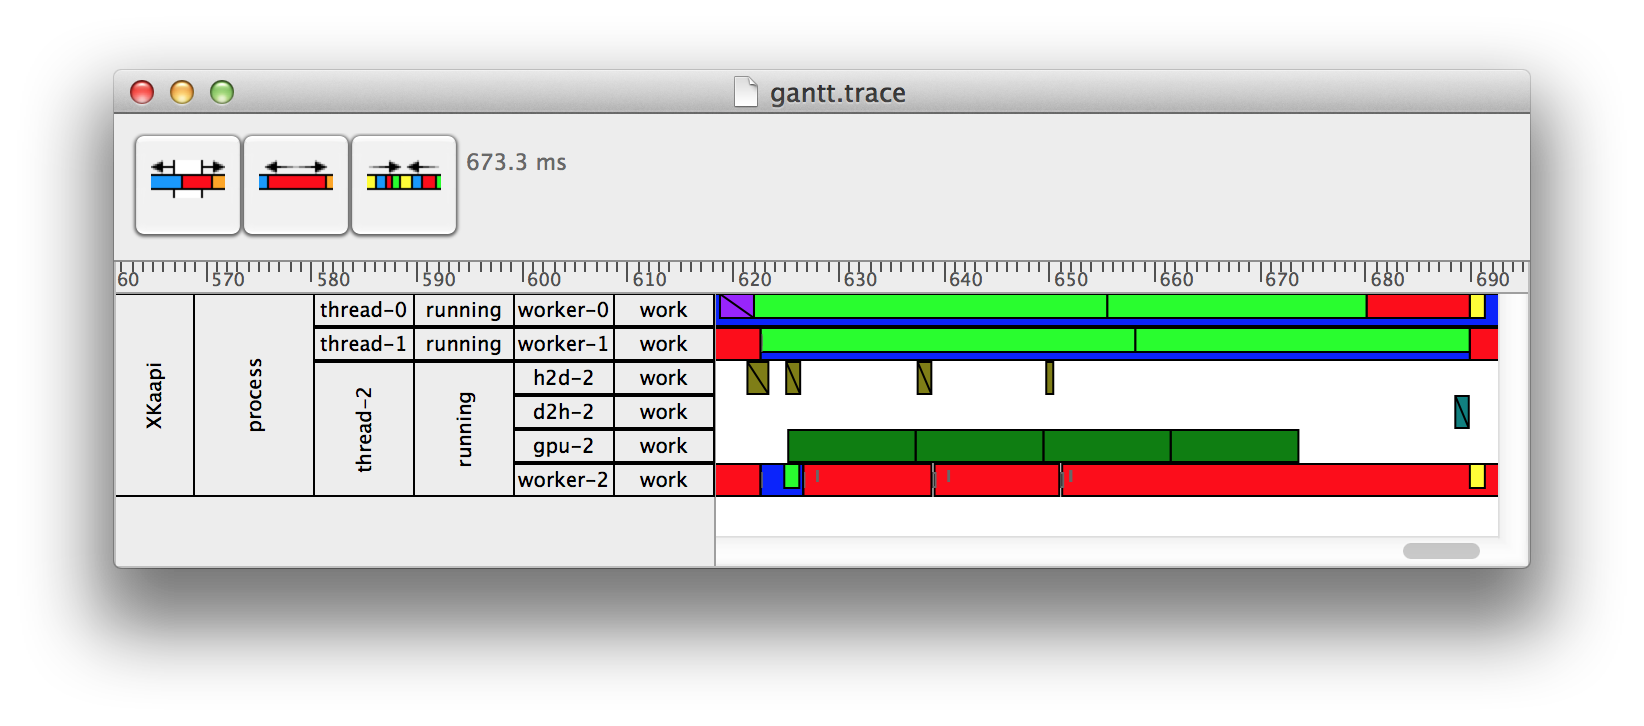
\includegraphics[scale=0.6]{sgemm-paje-trace.png}
\caption{
Gantt chart of a Paj\'e trace from a \kaapi SGEMM execution with two CPUs and one GPU.
}
\label{fig:trace}
\end{figure}

\definecolor{running}{rgb}{0.0,1.0,0.0}
\definecolor{idle}{rgb}{1.0,0.0,0.0}
\definecolor{active}{rgb}{0.0,0.0,1.0}
\definecolor{unroll}{rgb}{0.6,0.0,1.0}
\definecolor{kernel}{rgb}{0.0,0.5,0.0}
\definecolor{host2device}{rgb}{0.5,0.5,0.0}
\definecolor{device2host}{rgb}{0.0,0.5,0.5}
\definecolor{sync}{rgb}{1.0,1.0,0.0}
%\definecolor{}{rgb}{}

The colors from Figure \ref{fig:trace} represents the states:
\begin{itemize}
\item \textcolor{running}{running} tasks;
\item \textcolor{idle}{idle} state, which means it may request tasks by steal operations, or poll devices such as GPUs;
\item \textcolor{active}{active} state in which the runtime performs other activities as data validation;
\item \textcolor{unroll}{unroll} tasks to the acceleration structure used by \kaapi work stealing algorithm;
\item GPU \textcolor{kernel}{kernels};
\item GPU \textcolor{host2device}{host-to-device} transfers;
\item GPU \textcolor{device2host}{device-to-host} transfers;
\item memory \textcolor{sync}{synchronisation}.
\end{itemize}

We use arrows to illustrate steal request from thief, and reply from its victim. Here we ommited steal events for the sake of clarity.

\end{document}
